\chapter{Related work}

\section{Referential framework}

In this referential framework, we aim to provide a comprehensive overview of the key concepts necessary to understand the entirety of the project.

\subsection{The Speech Waveform}
We may sample the output of an analog microphone to produce speech signal. Using amplitude quantization along with sampling in the frequency domain, we will have a representation of the speech signal called the \textit{speech waveform}\cite{beigi2011speaker}.

\begin{figure}[htbp!]
    \centering
    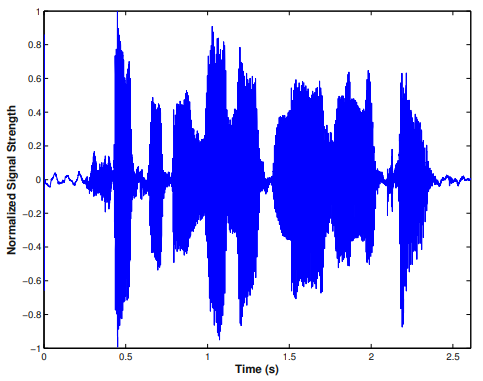
\includegraphics[height=5cm]{figures/speech_waveform.png}
    \caption{Illustration of Speech Waveform sampled at $f_s = 22050 Hz$ \cite{beigi2011speaker}.}
    \label{fig:wave_form}
\end{figure}

\subsection{Spectrogram}
A spectrogram is a three-dimensional representation of the spectral content of the speech signal. It represents the power of the different spectral components of each instance of speech. Spectrograms are images that represent sequences of spectra. Spectrogram is computed with Fourier Transform (FT) to transform a time domain signal into frequency domain signal. The whole signal is divided into individual windows(signal portions) and the FT is calculated for each window and join them back into a single image that shows the dominant frequencies in
each window \cite{sribhashyam2021pattern, wyse2017audio} as is shown in the Figure \ref{fig:spectrogram}.

\begin{figure}[htbp!]
    \centering
    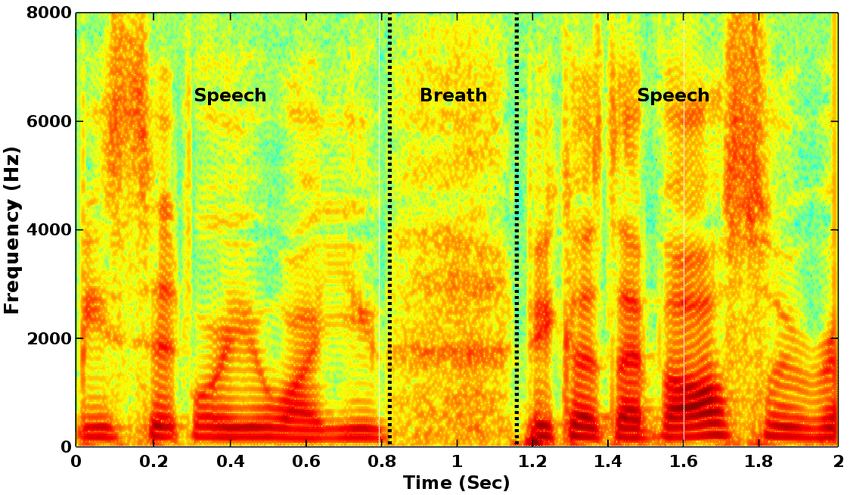
\includegraphics[height=6cm]{figures/spectogram.png}
    \caption{Illustration of Spectrogram of a speech signal with breath sound \cite{inproceedings}.}
    \label{fig:spectrogram}
\end{figure}


\subsection{Formants}
The formants of speech are resonant regions within the spectrogram. The vocal tract is changing shape so that the resonance is changing. the vocal tract length is inversely proportional to the height of the format in the frequency range of a speaker. Literature also showed that there are differences between male and female voices. The average female formant and fundamental frequencies are higher than that of the male speaking voice \cite{wu1991gender}. Formants are a frequency range where there is an absolute or relative maximum in the sound spectrum. The frequency at the maximum is the formant frequency\cite{pierce2019acoustics}. First formant, F1 corresponds to the vertical position of the tongue and is associated with frequencies between 200 and 900 Hz. Second formant, F2 corresponds to the horizontal position of the tongue and ranges from 600 - 2600 Hz \cite{watson1998acoustic}.

The vocal tract is changing shape so that the resonance is changing. The definition and estimation of formant locations is a difficult task. In general, the vocal tract length is inversely proportional to the height of the format in the frequency range of a speaker \cite{beigi2011speaker}.

\begin{figure}[htbp!]
    \centering
    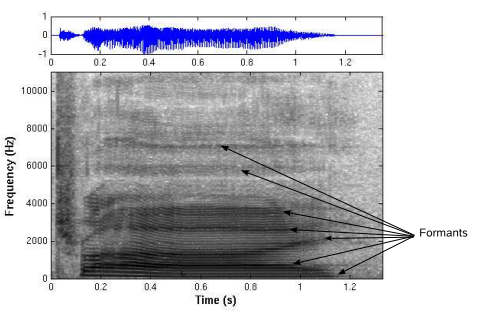
\includegraphics[height=6cm]{figures/formants.png}
    \caption{Illustration of Formants for an elongated utterance of the word \textit{try} \cite{beigi2011speaker}.}
    \label{fig:formants}
\end{figure}

\subsection{Vowel space}
The vowel space is a two-dimensional area bounded by the first and second formant frequency coordinates of vowels \cite{sandoval2013automatic}. The \ac{VSA}, defined as the area of the quadrilateral formed by the four corner vowels when projected on the first two formant frequencies (F1 and F2), is often used to characterize speech motor control \cite{berisha2014characterizing} as is shown in the Figure \ref{fig:vowel}. one method to use is the analysis of the vowel space during speech model training, thereby providing the foundational knowledge for developing a method to visualise and evaluate speech synthesis model training \cite{abeysinghe2022visualising}.

Vowel Space can be used by researchers to visualise the speech model (or the spoofing model in our case) and develop an understanding of how well the model learns the characteristics of the database during training stages \cite{abeysinghe2022visualising}.

\begin{figure}[htbp!]
    \centering
    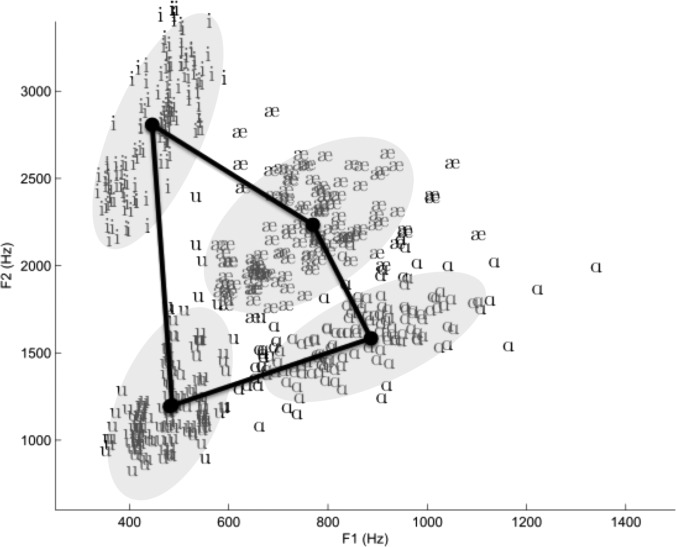
\includegraphics[height=6cm]{figures/vowel_space.png}
    \caption{Illustration of the first two formant frequencies for the four corner vowels \cite{berisha2014characterizing}.}
    \label{fig:vowel}
\end{figure}

\subsection{Speaker recognition}
Speech is an acoustic output produced by precisely coordinated movement of different human body parts. Therefore, there have been suggestions that acoustic features of speech can convey information about the physical characteristics of the speaker \cite{gupta2022estimation}.

It is important to note that speaker recognition in humans is not simply based on the apparent pitch content of the individual speaker’s utterances. It is a complex combination of many different features, some of which are quite simple to understand and seem very apparent, and others which are not well understood. The complex interactions between the two hemispheres of the brain in performing different tasks make matters much more complicated \cite{beigi2011speaker}.

\subsection{Error metrics and EER}

\begin{figure}[htbp!]
    \centering
    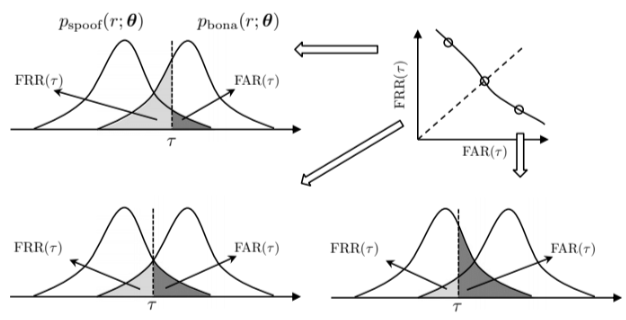
\includegraphics[height=6cm]{figures/eer.png}
    \caption{ Illustration of FRR($\tau$), FAR($\tau$), and DET curve \cite{wang2022practical}.}
    \label{fig:error}
\end{figure}

the classifier computes a score $r$ for the 
input trial and compares $r$ with a threshold $\tau$. The trial is classified as being
bonafide if $r \geq \tau$, otherwise
spoofed, two types of classification error can occur:

\begin{itemize}
    \item \textbf{False rejection}: falsely classifying a bona fide trial as being spoofed.
    \item \textbf{False acceptance}: falsely classifying a spoofed trial as being bona fide.
\end{itemize}

Without loss of generality, let us use \(p_{bona}(r;\theta)\) and \(P_{spoof}(r;\theta)\) to denote the score distributions of the bona fide and spoofed trials in a dataset, respectively.
The \(\theta\) denotes the trained parameter set of the PAD model. figure \ref{fig:error} illustrates examples of the score distributions. The classification threshold \(\tau\) marks the
region to claim bonafide and spoof. The shaded area of \(P_{bona}(r;\theta)\) on the left
side of \(\tau\) denotes false rejection. In contrast, the area of \(P_{spoof}(r;\theta)\) on the right side of \(\tau\) denotes false acceptance. Accordingly, the false rejection rate (FRR) and false acceptance rate (FAR) can be computed as 

\begin{equation}
    FRR(\tau) = \int_{-\infty}^{\tau} P_{bona}(r;\theta) \,dr
\end{equation}

\begin{equation}
    FAR(\tau) = \int_{\tau}^{\infty} P_{spoofed}(r;\theta) \,dr
\end{equation}

While being informative, the DET curve is not handy when a single metric is desired. One metric to summarize the discriminative power of the PAD model is the EER. In theory, EER refers to the joint between the DET curve and the anti-diagonal line (see the middle circle on the DET curve in Figure \ref{fig:error}). In practice the EER can be computed by:

\begin{equation}
    EER = \frac{FRR(\tau^{\prime}) + FAR(\tau^{\prime})}{2}
\end{equation}

\begin{equation}
    \tau^{\prime} = \underset{\tau}{\mathrm{arg min}} \ |FRR(\tau)-FAR(\tau)|
\end{equation}

\textit{An Example} of the calculation process for the EER will be provided next. Let's Suppose we have a dataset of 1000 attempts, consisting of 500 genuine attempts (legitimate users) and 500 impostor attempts (unauthorized users). We sort the scores in ascending order and calculate the False Acceptance Rate (FAR) and False Rejection Rate (FRR) at different thresholds. For simplicity, let's consider four thresholds: T1, T2, T3, and T4.

\begin{center}
    \begin{table}[h]
    \centering
        \begin{tabular}{| c | c | c | c |} 
             \hline
             Threshold ($T$) & Genuine ($FRR$) & Spoofing ($FAR$) & Equal Error Rate ($EER$) \\ [0.5ex] 
             \hline
             T1 & 0.0 & 1.0 & 0.5 \\ 
             \hline
             T2 & 0.1 & 0.5 & 0.3 \\
             \hline
             T3 & 0.3 & 0.2 & 0.25 \\
             \hline
             T4 & 0.5 & 0.05 & 0.275 \\
             \hline
        \end{tabular}
        \caption{Equal Error Rate example at different Thresholds.}
        \label{table:EER}
    \end{table}
\end{center}

To find the Equal Error Rate (EER), we look for the threshold where FAR and FRR are closest or equal. In this case, T3 has the closest values Therefore, the EER for this scenario would be the average of FAR and FRR at threshold T3. In this example, the Equal Error Rate is $25\%$. This means that at the threshold where FAR and FRR are equal, the system is expected to have a $25\%$ error rate, which is the average of false acceptance and false rejection rates.

\subsection{\acl{DFT}}

\begin{figure}[htbp!]
    \centering
    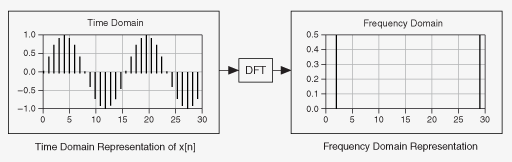
\includegraphics[height=4cm]{figures/dft.png}
    \caption{ Illustration of \ac{DFT} \cite{roberts2003lecture}.}
    \label{fig:dft}
\end{figure}

The Discrete \ac{DFT} is the equivalent of the continuous Fourier Transform for signals known only at $N$ instants separated by sample $T$ times (i.e. a finite sequence of data). The Fourier Transform of the original signal, $f(t)$, would be \cite{roberts2003lecture}:

\begin{equation}
    F(jw) = \int_{-\infty}^{\infty} f(t)e^{-jwt} \,dt
\end{equation}

We could regard each sample $f[k]$ as an impulse having area $f[k]$. Then, since the integrator exists only at the sample points:

\begin{equation}
    F(jw) = \sum_{k=0}^{N-1} f[k]e^{-jwt}
\end{equation}

We could in principle evaluate this for any $w$, but with only $N$ data points to start with, only $N$ final outputs will be significant\cite{roberts2003lecture}.

\subsection{\acl{MFCC}}

MFCC is a feature extraction technique that segment the signal applying the \ac{DFT}, taking the log of the magnitude, and then warping the frequencies on a Mel scale, followed by applying the \ac{IDCT}. Mel spectrum is computed by passing the Fourier transformed signal through a set of band-pass filters known as Mel-filter bank as is shown in the Figure \ref{fig:mel-filter}. A Mel is a unit of measure based on the human ears perceived frequency \cite{rao2017speech}.

\begin{figure}[htbp!]
    \centering
    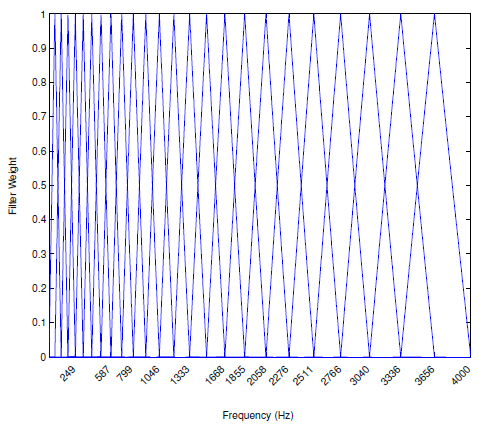
\includegraphics[height=6.3cm]{figures/mel-filter-bank.png}
    \caption{ Illustration of Mel-filter Bank \cite{beigi2011speaker}.}
    \label{fig:mel-filter}
\end{figure}

\section{State of the art}

\subsection{Taxonomy}
The taxonomy employed for classifying documents to the state of the art consists of two key fronts: existing voice anti-spoofing datasets and developed anti-spoofing models. These fronts served as the primary areas of focus during our information gathering process.

\subsubsection{Datasets}

Spoofing Attacks that we can find in the different datasets are \ac{LA}, \ac{PA} and \ac{DF}, and languages availables are \ac{ES} and \ac{EN}.

\begin{table}[h]
\centering
    \begin{tabular}{| c | c | c | c |} 
         \hline
         \textbf{Dataset} & \textbf{Languages} & \textbf{Spoofing Attacks} & \textbf{Reference} \\ [0.5ex] 
         \hline
         \hline
         PA Tamayo &  \acs{ES} & \acs{LA} & \cite{wang2022practical} \\ 
         \hline
         ASVSpoof 2015 & \acs{EN} & \acs{LA}, \acs{PA} & \cite{tamayo2022voice} \\ 
         \hline
         ASVSpoof 2017 & \acs{EN} & \acs{LA}, \acs{PA} & \cite{kinnunen17_interspeech} \\ 
         \hline
         ASVSpoof 2019 & \acs{EN} & \acs{LA}, \acs{PA} & \cite{yamagishi2019asvspoof} \\
         \hline
         ASVSpoof 2021 & \acs{EN} & \acs{LA}, \acs{PA}, \acs{DF} & \cite{delgado2021asvspoof} \\ 
         \hline
         SAS & \acs{EN} & \acs{LA} & \cite{wu2016anti} \\
         \hline
         FoR & \acs{EN} & \acs{LA} & \cite{reimao2019dataset} \\
         \hline
         VCTK & \acs{EN} & \acs{LA} & \cite{yamagishi2019cstr} \\
         \hline
         BTAS & \acs{EN} & \ac{PA} & \cite{korshunov2016overview} \\
         \hline
    \end{tabular}
    \caption{Datasets papers Taxonomy.}
    \label{table:datasets-taxonomy}
\end{table}

\subsubsection{Anti-spoofing models}

Front end types that we can find are Spectrogram, \ac{GD}, raw wave, \ac{LFCC}, \ac{RNN}, \ac{CQCC}, \ac{VAE} and models like ConvRBM and ResNet. And in terms of Back ends we could find \ac{CNN}, \ac{RNN}, \ac{LCNN}, \ac{GMM} and models like ResNet, ResNet2 and SENet34

\begin{center}
    \begin{table}[h]
    \centering
        \begin{tabular}{| c | c | c | c |} 
            \hline
            \textbf{Front end} & \textbf{Back end} & \textbf{Type} & \textbf{Reference} \\ [0.5ex] 
            \hline
            \hline
            Spectrogram & \acs{CNN} + \acs{RNN} & \makecell{Length-agnostic \\ \& Fixed input} & \cite{zhang2017investigation} \\ 
            \acs{GD} & \acs{CNN} & Segment level & \cite{tian2016spoofing} \\ 
            Wave & \acs{CNN} \acs{SLP} \& \acs{MLP} & Segment level & \cite{muckenhirn2017end} \\
            Wave + ConvRBM & \acs{GMM} & - & \cite{sailor2017unsupervised} \\ 
            Spec + \ac{DNN}(IGFCC) & \acs{GMM} & - & \cite{yu2017dnn} \\
            STFT \& MGD + GRCNN & PLAD & Utterance level & \cite{gomez2019gated} \\
            \hline
            \acs{GD} & ResNet+GAM att. &  Fixed input & \cite{tom2018end} \\
            IMFCC \& \acs{LFCC} & \acs{GMM} \& TDNN & Frame level & \cite{wu2014study} \\
            \acs{CQCC} \& Spectrogram & \acs{GMM} \& ResNet & Frame level & \cite{cai2017countermeasures} \\
            Spec. + \acs{LCNN} - \acs{RNN} & \acs{GMM} & - & \cite{lavrentyeva2017audio} \\
            \acs{CQCC} & ResNet & Frame level & \cite{chen2017resnet} \\
            \hline
            Spectrogram & \acs{CNN} & Fixed input size & \cite{chettri2019ensemble} \\
            \acs{CQT} + \acs{VAE} & CGCRNN & Length-agnostic & \cite{yang2019sjtu} \\
            Spectogram & SENet34 & Fixed input & \cite{lai2019assert} \\
            \acs{LFB} + ResNet & MLP & Utterance level & \cite{chen2020generalization} \\
            Wave & RawNet2 &  Fixed input size & \cite{tak2021end} \\
            \hline
        \end{tabular}
        \caption{Anti-Spoofing models Taxonomy.}
        \label{table:anti-spoofing-taxonomy}
    \end{table}
\end{center}

\subsection{Logical Access Presentation Attack}

Presentation attack mounted at the transmission point can use \ac{TTS} or \ac{VC} systems to produce the speech waveform of a target speaker. While the algorithms vary in detail, both \acs{TTS} and \acs{VC} can be written as a mapping function that converts one data sequence into another\cite{wang2022practical}. They can use specific models to convert the input into an acoustic feature for instance a sequence to convert the input text into a Mel-spectrogram \cite{shen2018natural}.

\subsection{Font End}

\subsubsection{DSP-based Deterministic Approaches}

Many front ends are based on \ac{DSP} algorithms that extract a sequence of acoustic features. Many speech processing tasks have used \ac{MFCC} \cite{davis1980comparison}. \ac{LFCC} \cite{davis1980comparison} and \ac{IMFCC} are closed related to the MFCC, but they use a different frequency scale and emphasize different frequency bands of the input waveform. Another popular front end is the \ac{CQCC} that uses \ac{CQT} rather than \ac{STFT}. Both \acs{CQCC} and \acs{LFCC} have been used in the ASVspoof challenges and are open-sourced. Rather than using cepstrum coefficients, many front ends only extract the spectrogram. Different from the cepstrum coefficients, \ac{LFB} compresses the spectrogram without cepstral analysis \cite{wang2022practical}.

\subsubsection{NN-based Supervised Training Approach}

\ac{DNN} can be used as a front end Different from a DSP-based one,  DNN-based front end has to be learned from the data. Such a trainable front end is preferred for three reasons. First, the DNN could be configured to extract acoustic features from a longer waveform segment. Second, the data-driven DNN with non-linear transformations is more powerful than linear operations in DSP-based front ends. Third, a DNN-based front end can easily be integrated with a DSP-based front end\cite{wang2022practical}. 

\subsubsection{DNN-based Self-supervised Training Approach}

It is also possible to apply self-supervised training to the DNN-based front end. One advantage is that a large amount of data can be used even if they do not have target labels. This is a popular topic in speech processing community, and many models have been proposed: wav2vec \cite{schneider2019wav2vec}, wav2vec2 \cite{baevski2020wav2vec}, VQ-wav2vec \cite{baevski2019vq},
contrastive predictive coding \cite{chung2021similarity}, auto-regressive predictive coding \cite{chung2021similarity}, and
HuBERT \cite{hsu2021hubert, wang2022practical}. 


\subsection{Back End}

\subsubsection{DNNs with Discriminative Training}

Many advanced PAD models use DNN-based back ends. A major sub-category is a \acs{DNN} with a discriminative training strategy. Given the target label \(y\) of input waveform  \(o_{1:T}\), the \acs{DNN} is directly trained to maximize the probability \(P(y|o_{1:T};\theta_{3})\). We use \(\theta_3\) to denote the parameter set of the DNN-based back end so that it can be differentiated from \((\theta_{1},\theta_{2})\) of the DNN-based front end. The topology of the DNN is a designer’s choice\cite{wang2022practical}.

\begin{figure}[htbp!]
    \centering
    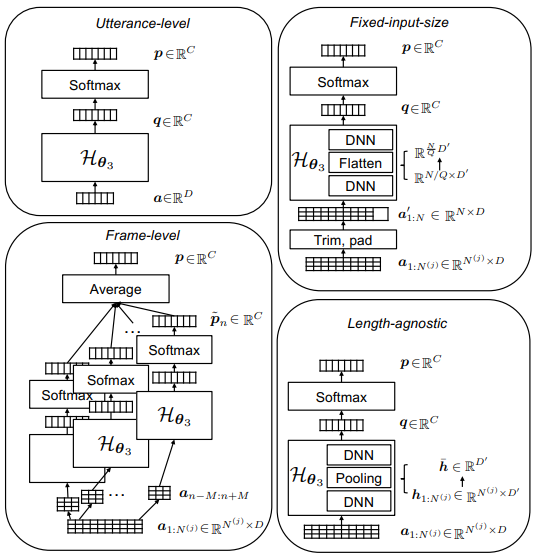
\includegraphics{figures/backends.png}
    \caption{  Illustration of different types of back ends \cite{wang2022practical}.}
    \label{fig:mel-filter}
\end{figure}

\subsubsection{Utterance-level Back End}
Given an utterance-level feature $\alpha = F_{\theta_1}(O_{1:T}) \in R^{D}$, from a trained front end $F_{\theta_1}$ the \acs{DNN} $H_{\theta_3}$ in the back end first converts $\alpha$ into an activation vector $q = H_{\theta_3}(\alpha) \in R^{C}$ After that, the vector $q$ is converted into $p = Softmax(H_{\theta_3}(\alpha))$.

Many types of DNNs can be used as the utterance-level back a network with a single fully-connected layer is used to convert the utterance-level embedding into the probability vector $p$ and the model achieved good performance \cite{wang2022practical}.

\subsubsection{Frame-level Back End}

When the output of the front end for the $j^{th}$ waveform is a sequence of acoustic features, the back end has to convert the sequence into the probability vector $p^{(j)} \in R^{C}$. The conversion process can be conducted using a frame-level back end with two parts. The first part is a DNN that converts into a sequence of probability vectors. The second part is
simple averaging that produces \cite{wang2022practical}.

\subsubsection{Segment-level Back End}

The segment-level back end is closely related to the frame-level back end. The difference is that the DNN can reduce the temporal resolution of the output sequence by a factor $Q$. The reduction of temporal resolution, or down-sampling, can be easily implemented using 1D convolution with a larger stride or local pooling operation \cite{wang2022practical}.

A potential advantage of the segment-level back end is that it ‘extracts useful information from a long temporal span without concatenating a large number of neighboring frames \cite{tian2016spoofing}.

\subsubsection{Fixed-input-size Back End}

Advanced DNNs such as ResNet and LCNN were originally proposed for image processing tasks. They are designed to process images with a fixed height and width. When ResNet or LCNN is used in a frame-level PAD back end, its input data at each frame step has a fixed size and can be directly processed as an image. However, an additional step is required to average the DNN’s output $p_n$ at every frame step.

A disadvantage of the frame- or segment-level back end is that the output $p_n$ only depends on a fixed number of input frames. It is presumably better if the input can be directly converted into a single probability vector $p \in R^{C}$ for the whole input trial \cite{wang2022practical}.

\subsubsection{Length-agnostic Back End}

A more flexible way to handle varied-length input is to augment the DNN with an operation that can reduce the varied-length hidden feature sequence into a single vector \cite{wang2022practical}.

\subsection{End-to-end Models}

End-to-end models as a combination of a neural back end and a dummy front end. From another viewpoint, we can also split an end-to-end model into front and back ends. The term ‘end-to-end’ is based on the fact that the front and back ends are jointly trained\cite{wang2022practical}.

\subsection{State of the art Conclusion}

Within the realm of anti-spoofing, a significant body of work revolves around the utilization of front-end and back-end frameworks. These frameworks play a crucial role in combining various models, enabling iterative processes that involve the integration of front-end models with different back-end counterparts, and vice versa. However, it is worth noting that there is currently a limited amount of research focused on accent-based approaches, and the exploration of multi-language capabilities remains relatively unexplored.

This observation presents an intriguing opportunity to delve into this field and conduct further research. By examining the potential applications of accent-based anti-spoofing techniques and exploring the possibilities of multi-language capabilities. Through meticulous investigation and experimentation, we aim to uncover new insights and develop innovative solutions that address the challenges posed by accents and multi-lingual scenarios.

\endinput
